\documentclass[border=10pt]{standalone}
\usepackage[svgnames]{xcolor}
\usepackage{amsmath}
\usepackage{pgfplots}
\pgfplotsset{compat=newest}
\usepackage[sfdefault]{FiraSans}
\usepackage{FiraMono}
\renewcommand*\familydefault{\sfdefault}
\begin{document}
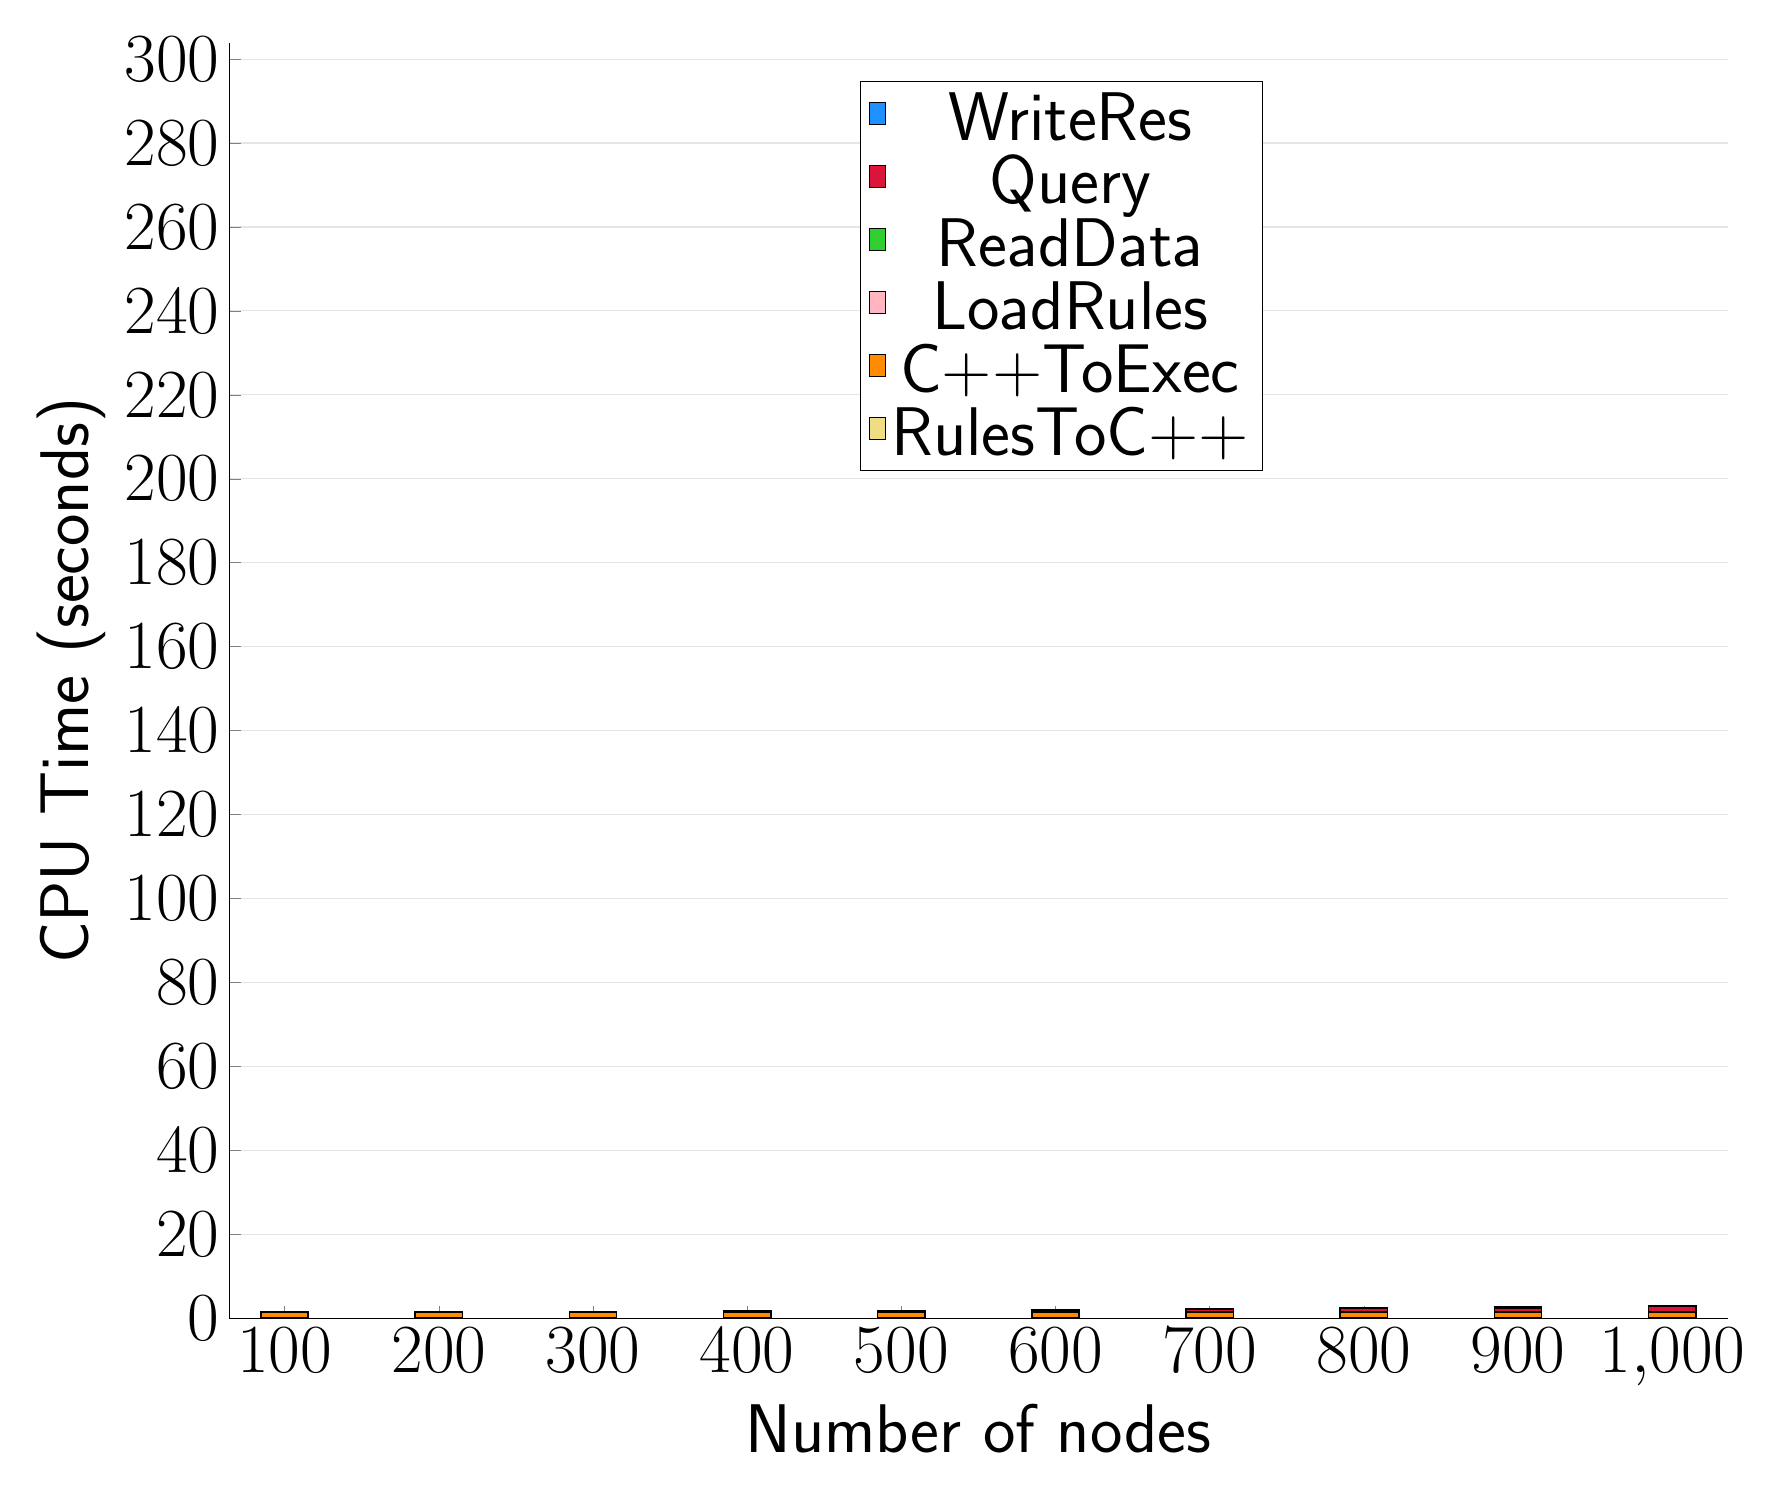
\begin{tikzpicture}
\begin{axis}[
   ybar stacked,
   width=1.7\textwidth,
   bar width=0.6cm,
   ymajorgrids, tick align=inside,
   major grid style={draw=gray!20},
   xtick=data,
   ymin=0, ymax=303.8692,
   axis x line*=bottom,
   axis y line*=left,
   enlarge x limits=0.04,
   legend style={
       at={(0.69, 0.97)},
       anchor=north east,
       legend columns=1,
       font=\Huge,
   },
   ylabel={CPU Time (seconds)},
   xlabel={Number of nodes},
   label style={font=\Huge},
   tick label style={font=\Huge},
]
\addlegendimage{fill=DodgerBlue, draw=black, line width=0.2pt}
\addlegendentry{WriteRes}
\addlegendimage{fill=Crimson, draw=black, line width=0.2pt}
\addlegendentry{Query}
\addlegendimage{fill=LimeGreen, draw=black, line width=0.2pt}
\addlegendentry{ReadData}
\addlegendimage{fill=LightPink, draw=black, line width=0.2pt}
\addlegendentry{LoadRules}
\addlegendimage{fill=DarkOrange, draw=black, line width=0.2pt}
\addlegendentry{C++ToExec}
\addlegendimage{fill=LightGoldenrod, draw=black, line width=0.2pt}
\addlegendentry{RulesToC++}
\addplot +[fill=LightGoldenrod, draw=black, line width=0.55pt] coordinates {
(100, 0.0020000000000000005)
(200, 0.006000000000000001)
(300, 0.0020000000000000005)
(400, 0.0020000000000000005)
(500, 0.004000000000000001)
(600, 0.004000000000000001)
(700, 0.004000000000000001)
(800, 0.009999999999999998)
(900, 0.004000000000000001)
(1000, 0.008000000000000002)
};
\addplot +[fill=DarkOrange, draw=black, line width=0.55pt] coordinates {
(100, 1.48)
(200, 1.4739999999999998)
(300, 1.488)
(400, 1.482)
(500, 1.478)
(600, 1.478)
(700, 1.466)
(800, 1.4620000000000002)
(900, 1.4880000000000002)
(1000, 1.504)
};
\addplot +[fill=LightPink, draw=black, line width=0.55pt] coordinates {
(100, 0.0001692)
(200, 0.00016879999999999998)
(300, 0.000182)
(400, 0.0001746)
(500, 0.000169)
(600, 0.000168)
(700, 0.00016380000000000002)
(800, 0.00016439999999999998)
(900, 0.000166)
(1000, 0.0001592)
};
\addplot +[fill=LimeGreen, draw=black, line width=0.55pt] coordinates {
(100, 0.0007474)
(200, 0.0012067999999999998)
(300, 0.0016281999999999998)
(400, 0.0019854)
(500, 0.0023794000000000003)
(600, 0.0027480000000000004)
(700, 0.0028266000000000003)
(800, 0.0027815999999999995)
(900, 0.0037388000000000005)
(1000, 0.0029401999999999996)
};
\addplot +[fill=Crimson, draw=black, line width=0.55pt] coordinates {
(100, 0.020999999999999998)
(200, 0.06437040000000001)
(300, 0.1214092)
(400, 0.20174659999999997)
(500, 0.3090962)
(600, 0.4413768)
(700, 0.5979896)
(800, 0.7903472)
(900, 1.006362)
(1000, 1.2769679999999999)
};
\addplot +[fill=DodgerBlue, draw=black, line width=0.55pt] coordinates {
(100, 0.0038366)
(200, 0.009382600000000001)
(300, 0.019478600000000002)
(400, 0.034334199999999995)
(500, 0.053332000000000004)
(600, 0.07630279999999999)
(700, 0.1045544)
(800, 0.137103)
(900, 0.1708554)
(1000, 0.21426239999999996)
};
\end{axis}
\end{tikzpicture}

\end{document}
